%%%%%%%%%%%%%%%%%%%%%%%%%%%%%%%%%%%%%%%%%%%%%%%%%%%%%%%%%%%%%%%%%%%%%%%%%%%

\documentclass{standalone}

\usepackage{amsmath}
\usepackage{mathptmx}
\usepackage{pgfplots}
\usetikzlibrary{external}
\tikzexternalize{spring-constant-frequency}
\pgfplotsset{compat=1.16}

%% IEEE uses Times Roman font, so we'll default to Times.
%% These three commands make up the entire times.sty package.
\renewcommand{\rmdefault}{ptm}
\renewcommand{\ttdefault}{pcr}
\normalfont\selectfont

\begin{document}

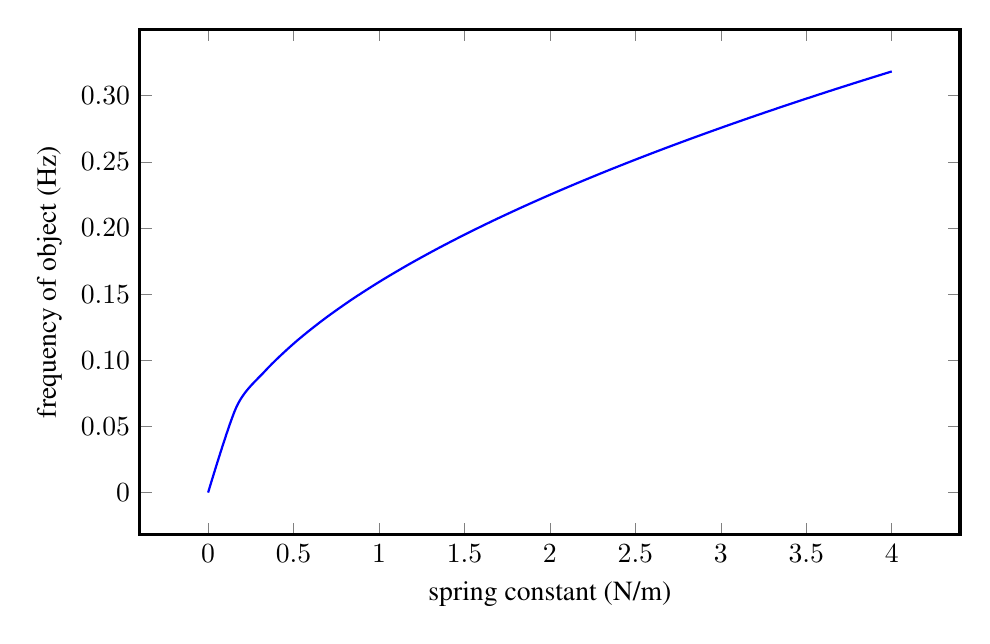
\begin{tikzpicture}
\tikzset{%%
  every mark/.append style={scale=1.0},%%
  scale=1.0%%
}
\pgfplotsset{%%
  every axis/.append style={font=\normalsize}%%
}
%%
\begin{axis}[%%
  axis line style=very thick,%%
  enlargelimits=true,%%
  height=8cm,%%
  plotStyle/.style={%%
    domain=0:4,%%
    mark=none,%%
    smooth,%%
    thick%%
  },%%
  width=12cm,%%
  %% x axis
  xlabel={\normalsize spring constant~(N/m)},%%
  %% y axis
  ylabel={\normalsize frequency of object~(Hz)},%%
  ytick={0,0.05,0.10,0.15,0.20,0.25,0.30},%%
  yticklabels={$0$,$0.05$,$0.10$,$0.15$,$0.20$,$0.25$,$0.30$}%%
]
%%
%%
%% Object mass = 1, vary the spring constant.
\addplot+ [plotStyle]
{(1 / (2*pi)) * sqrt(x / 1)};
\end{axis}
\end{tikzpicture}

\end{document}
